\documentclass[8pt,a4paper,landscape,oneside]{amsart}
\usepackage{amsmath, amsthm, amssymb, amsfonts}
\usepackage[T1]{fontenc}
\usepackage[utf8]{inputenc}
\usepackage{multicol}
\usepackage{fancyhdr}

%\usepackage{booktabs}
%\usepackage{caption}
%\usepackage{color}
%\usepackage{float}
\usepackage{fullpage}
%\usepackage{subcaption}
%\usepackage[scaled]{beramono}
\usepackage{titling}
%\usepackage{datetime}
%\usepackage{enumitem}
%\usepackage{bm}
\usepackage{fontspec}
\usepackage{graphicx}

% Minted
\usepackage{minted}
\newcommand{\code}[1]{\inputminted[fontsize=\normalsize,baselinestretch=1]{java}{code/#1}}

\newcommand{\bigO}{\mathcal{O}}

% Define flip table command, may only work on windows
\newfontfamily{\fliptablefont}{Arial Unicode MS}
\DeclareRobustCommand{\fliptable}{{\fliptablefont ┻━┻ ︵ \( °□° )/ ︵ ┻━┻ }}

\pagestyle{fancy}
\lhead{\fliptable - Lund University}
\rhead{\thepage}
\cfoot{}
\setlength{\headheight}{15.2pt}
\setlength{\droptitle}{-20pt}
\posttitle{\par\end{center}}
\renewcommand{\headrulewidth}{0.4pt}
\renewcommand{\footrulewidth}{0.4pt}

\begin{document}

\begin{multicols*}{3}
%\maketitle
\thispagestyle{fancy}
\vspace{-3em}

\tableofcontents

\section{Math}
  \subsection{Trigonometry}
  Common formulas for sin and cos.
  \begin{center}
  \begin{tabular}{rcl}
  \hline
  $\tan x$ & = & $\frac{\sin x}{\cos x}$ \\
  $\sin(-x)$ & = & $-\sin x$ \\
  $\cos(-x)$ & = & $\cos x$ \\
  $\sin(\pi/2-x)$ & = & $\cos x$ \\
  $\cos(\pi/2-x)$ & = & $\sin x$ \\
  $\sin(\pi-x)$ & = & $\sin x$ \\
  $\cos(\pi-x)$ & = & $-\cos x$ \\
  \hline
  $\sin(\alpha+\beta)$ & = & $\sin\alpha \cdot \cos\beta + \cos\alpha \cdot \sin\beta$ \\
  $\cos(\alpha+\beta)$ & = & $\cos\alpha \cdot \cos\beta - \sin\alpha \cdot \sin\beta$ \\
  $\sin(\alpha-\beta)$ & = & $\sin\alpha \cdot \cos\beta - \cos\alpha \cdot \sin\beta$ \\
  $\cos(\alpha-\beta)$ & = & $\cos\alpha \cdot \cos\beta + \sin\alpha \cdot \sin\beta$ \\
  \hline
  $\sin 2x$ & = & $2 \cdot \sin x \cdot \cos x$ \\
  $\cos 2x$ & = & $\cos^2 x - \sin^2 x$ \\
  $2 \cdot \sin x \cdot \sin y$ & = & $\cos(x-y) - \cos(x+y)$ \\
  $2 \cdot \cos x \cdot \cos y$ & = & $\cos(x-y) + \cos(x+y)$ \\
  $2 \cdot \sin x \cdot \cos y$ & = & $\sin(x-y) + \sin(x+y)$ \\ \hline
  \end{tabular}
  \end{center}

  \subsection{Geometry}
  \textit{Given a triangle $\mathit{abc, u = a \rightarrow b, v = a \rightarrow c}$}

  \textbf{Cross product:} 

  $u \times v = u_xv_y - u_yv_x$
  \newline

  \textbf{Dot product:} 

  $u \cdot v = u_xv_x + u_yv_y$
  \newline

  \textbf{Orthogonal projection:} 

  $u' = \frac{u \cdot v}{|v^2|}v$
  \newline

  \textbf{Angle between vectors [-pi, pi]:} 

  $\mathrm{atan2} (u \times v, u \cdot v) = $

  $\mathrm{atan2} (c_y - a_y, c_x - a_x) - \mathrm{atan2} (b_y - a_y, b_x - a_x)$
  \newline

  \textbf{Triangle area:} 

  $\frac{1}{2}(u \times v) = \frac{1}{2}((b-a) \times (c-a))$
  \newline

  \textbf{Polygon area:} 

  $A = \frac{1}{2}\sum\limits^{n-1}_{i=0}(x_iy_{i+1}-x_{i+1}y_i)$

  (where $n$ is \#vertices)
  \newline

  \textbf{Polygon center:}

  $C_x = \frac{1}{6A}\sum\limits^{n-1}_{i=0}(x_i+x_{i+1})(x_iy_{i+1}-x_{i+1}y_i)$

  $C_y = \frac{1}{6A}\sum\limits^{n-1}_{i=0}(y_i+y_{i+1})(x_iy_{i+1}-x_{i+1}y_i)$
  \newline

  \textbf{Point inside polygon:} 

  $S = \sum\limits^{n-2}_{i=0}\mathrm{angle}(p - v_i, p - v_{i+1}) + \mathrm{angle}(p - v_{n-1}, p - v_0)$

  $\mathrm{if} (S == \pm 2k\pi)$: inside

  $\mathrm{if} (S == 0)$: outside

  (where $p$ is a point)

  A faster way to calculate would be using raycasting and counting intersecting edges.
  
  \subsection{Combinatorics}
  Various useful combinatoric formulas.
  Formulas for the number of ways of taking $k$ from $n$ items:
  \begin{center}
  \begin{tabular}{|c|c|c|} \hline
  & With repetitions & No repetitions \\
  \hline
  Order matters & $n^k$ & $\frac{n!}{(n-k)!}$ \\ \hline
  Any order & $\binom{n+k-1}{k}$ & $\binom{n}{k} = \frac{n!}{k!\cdot(n-k)!}$ \\ \hline
  \end{tabular}
  \end{center}
  Formulas progressions and sums of arithmetic and geometric sequences:
  \begin{center}
  \begin{tabular}{|c|c|c|} \hline
  & Arithmetic & Geometric \\
  \hline
  Progression & \shortstack{$a_n = a_{n-1} + d =$ \\ $a_1 + d\cdot(n-1)$} & \shortstack{$a_n = a_{n-1}\cdot r =$ \\ $a_1\cdot r^{n-1}$} \\ \hline
  Sum & $S_n = \frac{n(a_1+a_n)}{2}$ & $S_n = \frac{a(r^n-1)}{r-1}$ \\ \hline
  \end{tabular}
  \end{center}
  
  \subsection{Number Theory}
  Various useful number theory formulas.
  \code{Math/Gcd.java}


\section{Algorithmic concepts}
  \subsection{Inclusion-Exclusion principle}
  This principle may be useful for problems that you can model as $k$ overlapping subsets over $n$ values, where you are interested in finding the union of the $k$ subsets.
  
  An example of this may be "Find the amount of numbers between $1$ and $2^{30}$ that are divisible by neither 2, 3 nor 5". Model this as three sets $A$, $B$ and $C$ representing numbers from $[1, 2^{30}]$ not divisible by 2, 3 and 5. Calculate the following:
  \[
  \begin{split}
  |A \cup B \cup C| = & |A| + |B| + |C| - |A \cap B| - |A \cap C| \\
  & - |B \cap C| + |A \cap B \cap C|
  \end{split}
  \]
  This is visualized in Figure ~\ref{inclusion-exclusion} below. Note that all intersections with an even amount of terms will be negative, even in the general case with $k$ sets.
  
  These types of problems are characterized by \emph{huge output} (often modulo $m$) and \emph{few subsets} $k$.
  
  \begin{figure}[H]
  \centering
   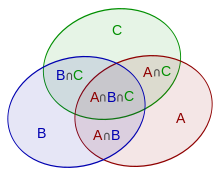
\includegraphics[scale=0.5]{inclusion-exclusion_principle.png}
   \caption{The three sets visualized, gives intuition about why we need to subtract even terms and add odd ones.}
   \label{inclusion-exclusion}
  \end{figure}
  
  \subsection{Meet in the middle}
  This method is useful for problems that are a little too large to be brute forced and have a structure that allows it to be split. 
  
  An example of this may be "Given an array of $n \in [1, 2^{36}]$ numbers find the maximum subset sum modulo $m$". Naively testing the sum of all subsets will not work ($2^{36}$ is too large), instead split the array in two and find all possible sums in each half (only $2^{18}$ in each). When this is done we merge them in a smart way that is faster than $\bigO(n^2)$.
  
  These types of problems are characterized by an \emph{input size} just beyond the range of brute force and \emph{easily partitioned} data.


\section{Code Templates}
  \subsection{KattIO}
  \code{Kattio.java}
  
  
\section{Search \& Sort}
  \subsection{Binary Search}
  Time complexity is $\bigO(n \log n)$ and space complexity is $\bigO(1)$.
  \code{Structures/BinarySearch.java}
  \subsection{Sorting}
  Time complexity is $\bigO(n \log n)$ for both algorithms and space complexity is $\bigO(\log n)$.
  \begin{itemize}
  \item \texttt{Collections.sort()} uses Merge Sort
  \item \texttt{Arrays.sort()} uses Quick Sort
  \end{itemize}
  
  \subsection{Quick Select}
  Time complexity is $\bigO(n)$ on average and $\bigO(n^2)$ in the worst case. The space complexity is $\bigO(\log n)$.
  \code{Structures/QuickSelect.java}
  
  \subsection{Knuth-Morris-Pratt Algorithm}
  Time complexity is $\bigO(n)$ and space complexity is $\bigO(\log n)$. Good when the alphabet is small (around 4-5 characters).
  \code{Structures/KMP.java}
  
  \subsection{Z-Array Algorithm}
  Time complexity is $\bigO(n)$ and space complexity is $\bigO(n)$. Good when the alphabet is large.
  \code{Structures/ZArray.java}
  
  
\section{Data Structures}
  \subsection{Fenwick tree}
  Time complexity is $\bigO(\log n)$ for all operations and space complexity is $\bigO(1)$.
  \code{Structures/Fenwick.java}
  
  \subsection{Segment Tree}
  Time complexity is $\bigO(n)$ for construction and $\bigO(\log n)$ for all operations and space complexity is $\bigO(n)$.
  \code{Structures/SegmentTreeRMQ.java}
  
  \subsection{Monotone Queue}
  Time complexity is amortized $\bigO(1)$ for all operations and space complexity is $\bigO(w)$, where $w$ is the size of the sliding window.
  \code{Structures/MinMonoQueue.java}
  
  \subsection{Union-Find}
  Time complexity is amortized $\bigO(\log^*{n})$ for all operations and space complexity is $\bigO(1)$.
  \code{Structures/UnionFind.java}
  
  \subsection{Suffix Array}
  Time complexity for construction is $\bigO(n\log{n}\log{n})$ and space complexity is $\bigO(n)$.
  \code{Structures/SuffixArray.java}
  
  \subsection{Treap}
  Time complexity for construction is $\bigO(n)$, for all operations $\bigO(\log{n})$ and space complexity is $\bigO(n)$.
  \code{Structures/Treap.java}
  
  
\section{Graph Algorithms}
  \subsection{Graph definition}
  This graph class is used for the graph algorithms. Not all attributes of the classes are needed in all problems.
  \code{Graphs/Graph.java}
  
  \subsection{Dijsktra's Algorithm}
  Time complexity is $\bigO(|E| \log{|V|})$ and space complexity is $\bigO(|V|)$.
  \code{Graphs/Dijkstras.java}
  
  \subsection{Bellman-Ford Algorithm}
  Time complexity is $\bigO(|E||V|)$ and space complexity is $\bigO(|V|)$.
  \code{Graphs/BellmanFord.java}
  
  \subsection{Floyd-Warshall Algorithm}
  Time complexity is $\bigO(|V|^3)$ and space complexity is $\bigO(|V|^2)$.
  \code{Graphs/FloydWarshall.java}
  
  \subsection{Prim's Algorithm}
  Time complexity is $\bigO(|E| \log{|V|})$ and space complexity is $\bigO(|V|)$.
  \code{Graphs/MST.java}
  
  \subsection{Topological Sort}
  Time complexity is $\bigO(|E| + |V|)$ and space complexity is $\bigO(|V|)$. You need to pop the resulting stack to get the nodes in the correct order, \textit{do not} loop over it/convert to list since that results in the reverse order. Running this on a graph with cycles yields an incorrect result.
  \code{Graphs/TopologicalSort.java}
  
  \subsection{Network Flow/Min Cut}
  Time complexity is $\bigO(|V||E|^2)$ and space complexity is $\bigO(|V|+|E|)$. Solves both max flow and min cut. If the graph is very large this can be improved to $\bigO(|E|^2 \log{C})$ (where C is the maximum flow). Find $\Delta$, the largest POT that is smaller than the largest flow out of $s$. Run the algorithm but only allow edges with a capacity of at least $\Delta$. When there are no more paths between $s$ and $t$ let $\Delta = \Delta / 2$ and repeat until $\Delta < 0$.
  \code{Graphs/NetworkFlow.java}
  
  \subsection{Hopcroft-Carp Algorithm}
  Time complexity is $\bigO(|E|\sqrt{|V|})$ and space complexity is $\bigO(|V|)$. Gives both a maximum bipartite matching and a minimum vertex cover. Can be converted to Maximum Independent Set by selecting all vertices not in the vertex cover.
  \code{Graphs/HopcroftCarp.java}
  
  
\section{Geometry}
  \subsection{Graham Scan}
  Time complexity is $\bigO(n\log{n})$ and space complexity is $\bigO(n)$.
  \code{Geometry/GrahamScan.java}
  
\section{Dynamic Programing}
  \subsection{Knapsack 1/0}
  Given a set of items each with a value $v_i$ and a weight $w_i$ you want to maximize the value while limited by a total weight $W$. The following recursion relation solves the problem in $\bigO(nW)$:
  \[
  Opt(i,W) = \begin{cases}
  0 & \text{if } i=0 \\
  Opt(i-1,W) & \text{if } W<w_i \\
  \begin{aligned}[t]\arraycolsep=0pt
    \max\lbrace &
      Opt(i-1,W), \\ &
      Opt(i-1,W-w_i) + v_i \rbrace
  \end{aligned} & \text{if } W \geq w_i
  \end{cases}
  \]
  The answer is $Opt(n, W)$.
  
  \subsection{Knapsack Unbounded}
  The same problem as above but with an unlimited amount of each item. The following recursion relation solves the problem in $\bigO(nW)$:
  \[
  Opt(W) = \begin{cases}
  0 & \text{if } W=0 \\
  \max\limits_{w_i \leq W} \lbrace Opt(W-w_i) + v_i \rbrace & \text{otherwise}
  \end{cases}
  \]
  The answer is $Opt(W)$.
  
  \subsection{Subset Sum}
  \label{subset-sum}
  Given a set of values you want to select a subset that sum to $W$. This is solved by knapsack by letting $w_i = v_i$ and checking if $Opt(n, W) = W$.
  
  \subsection{Minimum Partition Distance}
  Given a set of $n$ numbers $s_i$ you want to split them into two sets $A$ and $B$ such that $|\sum a_i| - |\sum b_i|$ is minimized. The following recursion relation solves the problem in $\bigO(nS)$ (where $S$ is the sum of all numbers):
  \[
  Opt(i,d) = \begin{cases}
  d & \text{if } i=0 \\
  \begin{aligned}[t]\arraycolsep=0pt
    \arg\min\limits_x(x \in \{ & Opt(i-1,d-s_i), \\ &
    Opt(i-1,d+s_i)\} : |x|)
  \end{aligned} & \text{if } i > 0 \\
  
  \end{cases}
  \]
  The answer is $Opt(n, 0)$.
  
  \subsection{Edit distance}
  Given two strings $a$ and $b$ of length $m$ and $n$ find the minimum edit distance using penalties $p_m$ for mismatches and $p_s$ when padding with spaces. The following recursion relation solves the problem in $\bigO(mn)$:
  \[
  Opt(i,j) = \begin{cases}
  j*p_s & \text{if } i=0 \\
  i*p_s & \text{if } j=0 \\
  Opt(i-1,j-1) & \text{if } a_i=b_j \\
  \begin{aligned}[t]\arraycolsep=0pt
    \min\lbrace &
      Opt(i-1,j-1) + p_m, \\ &
      Opt(i-1,j) + p_s, \\ & 
      Opt(i,j-1) + p_s \rbrace
  \end{aligned} & \text{if } a_i\neq b_j
  \end{cases}
  \]
  The answer is $Opt(m,n)$. Example: ED("ABC", "ACD") = 2 ("ABC-" vs. "A-CD") where $p_m = p_s = 1$.
  
  \subsection{Longest Common Subsequence}
  Related to edit distance, you want to compute the longest common subsequence of two strings $a$ and $b$ of length $m$ and $n$. The result of the algorithm is the string itself ($\frown$ appends to the result). The following recursion relation solves the problem in $\bigO(mn)$:
  \[
  Opt(i,j) = \begin{cases}
  0 & \text{if } i=0 \text{ or } j=0 \\
  Opt(i-1,j-1) \frown a_i & \text{if } a_i=b_j \\
  \begin{aligned}[t]\arraycolsep=0pt
    \mathrm{longest}\lbrace &
      Opt(i-1,j), \\ & 
      Opt(i,j-1) \rbrace
  \end{aligned} & \text{if } a_i\neq b_j
  \end{cases}
  \]
  The answer is $Opt(m,n)$. Example: LCS("ABCD", "A-B-D-C") = "ABD".
  
  \subsection{Longest Increasing Subsequence}
  Time complexity is $\bigO(n\log n)$ and space complexity is $\bigO(n)$.
  \code{DP/LongestIncreasingSubsequence.java}
  
  
\section{Scheduling}
All the following problems consider the case where you get a list of $n$ tasks $t_i$ which may each have a start time $s_i$ an end time $e_i$ and a value $v_i$.
  \subsection{1 machine, maximum tasks}
  The goal is to maximize the amount of tasks done. Can be trivially solved by sorting the tasks by $e_i$ in ascending order and greedily pick as many as possible. Time complexity is $\bigO(n\log n)$.
  
  \subsection{1 machine, maximum time}
  The goal is to maximize the amount of time spent working during a timeslot of length $W$. The tasks have a duration but no start time. This is solved by dynamic programming like the subset sum problem (see~\ref{subset-sum}) by letting the task durations be the weights $w_i$.
  
  \subsection{1 machine, maximum value}
  The goal is to maximize the total value $V$ of all the tasks that are serviced. This is solved by first sorting by $e_i$ and then using dynamic programming. The following recursion relation solves the problem:
  \[
  Opt(i) = \begin{cases}
  0 & \text{if } i = 0 \\
  \max(v_i + Opt(p(i)), Opt(i-1)) & \text{if } i > 0
  \end{cases}
  \]
  Where $p(i)$ is the index of first task (backwards in time) that does not overlap with task $i$. The answer is $Opt(n)$ and the total time complexity is $\bigO(n\log n)$.
  
  \subsection{$k$ machines, maximum tasks}
  The goal is to maximize the amount of tasks done given $k$ machines. To solve this we first sort the tasks by $e_i$, then build a timeline of tasks as follows:
  \begin{enumerate}
    \item Pick a task and try to put it on the timeline.
    \item If it collides with a previous task add a new layer to the timeline and try to put it there, if it still collides add another layer, etcetera\ldots
    \item Return to the lowest level and go back to step 1.
  \end{enumerate}
  When this is done you have a timeline of multiple layers each with an amount of tasks. To get the solution sort the layers in the timeline by decreasing amount of tasks and assign the $k$ first layers to your machines. Time complexity is $\bigO(n\log n)$.
  
  \subsection{Minimize machines, all tasks}
  The goal is to minimize the amount of machines $k$ needed to service \emph{all} of the tasks. This can be solved by sorting the tasks by $s_i$ and finding the maximum depth $d$ (the maximum amount of simultaneous tasks). To solve it we need $k=d$ machines. To assign work go through the list and give each task to and idle machine.  Time complexity is $\bigO(n\log n)$.
        
        
\section{Checking for errors}
  \subsection{Wrong Answer}
    \begin{itemize}
    \item Test minimal input
    \item Integer overflow?
    \item Double precision too low?
    \item Reread the problem statement
    \item Look for edge-cases
    \item Start creating small testcases
    \end{itemize}
  \subsection{Time Limit Exceeded}
    \begin{itemize}
    \item Is the time complexity checked?
    \item Is the output efficient?
    \item If written in python, rewrite in java?
    \item Can we apply DP anywhere?
    \item Create worst case input
    \end{itemize}
  \subsection{Runtime Error}
    \begin{itemize}
    \item Stack overflow?
    \item Index out of bounds?
    \item Division by $0$?
    \item Concurrent modification?
    \end{itemize}
  \subsection{Memory Limit Exceeded}
    \begin{itemize}
    \item Create objects outside recursive function
    \item Convert recursive functions to iterative with your own stack
    \end{itemize}
        
        
\section{Running time}
The following table contains the number of elements that can be processed per second given the algorithm complexity in $n$.
\begin{center}
\begin{tabular}{lr}
Alg. Complexity & Input size/s \\ \hline
$\bigO(\log^*{n})$   & $\rightarrow \infty$ \\
$\bigO(\log{n})$     & 2 \textasciicircum 100 000 000 \\
$\bigO(n)$           & 100 000 000 \\
$\bigO(n*\log{n})$   & 4 500 000 \\
$\bigO(n*\log{n}*\log{n})$ & 300 000 \\
$\bigO(n^2)$         & 10 000 \\
$\bigO(n^2*\log{n})$ & 3 000 \\
$\bigO(n^3)$         & 450 \\
$\bigO(2^n)$         & 26.5 \\
$\bigO(3^n)$         & 16.5 \\
$\bigO(n!)$          & 10
\end{tabular}
\end{center}



\end{multicols*}
\end{document}
